\documentclass{article}
\usepackage[utf8]{inputenc}
\usepackage{graphicx}
\usepackage{subfloat}

\begin{document}
\title{Hands-on 18.05.2018 of the Computer Vision course at the
  University of Helsinki in May, 2018}

\author{\emph{Vladimir Dobrodeev, student number 014690820}}
\maketitle

\newpage

\section{Hands on}

\subsection{Disparity map}

The first task of this hands-on was to create a disparity map for two images, which are supposed to be captured from left and right camera of some stereo set-up. The disparity of pixels was checked first with using a detector created with \textit{StereoBM\_create}. This methods takes two parameters, which defined the way how the disparity is detected: \textit{numDisparities} and \textit{blockSize}. A set of experiments was conducted with different values of these parameters. Result disparity map is presented at a grayscale image together with left original image. Red pixels depict cases, where disparity could not be calculated.

Experiments showed, that for large block sizes too many the algorithm can not calculate disparity for a large share of pixels. For very large block sizes the whole map is painted with red. With decreasing of block size result disparity map looks less smooth but it is possible to see contours of objects. Varying numDisparsities has an important effect. When this parameter has a quite large value (160) there is an area at the left side, where disparity can not be calculated. It seems, that as search range for disparity is large, the method is not able to find any matching pixels lying in that area. If the parameter's value has the smallest value (16), this area is significantly diminished.

\begin{figure}[H]
	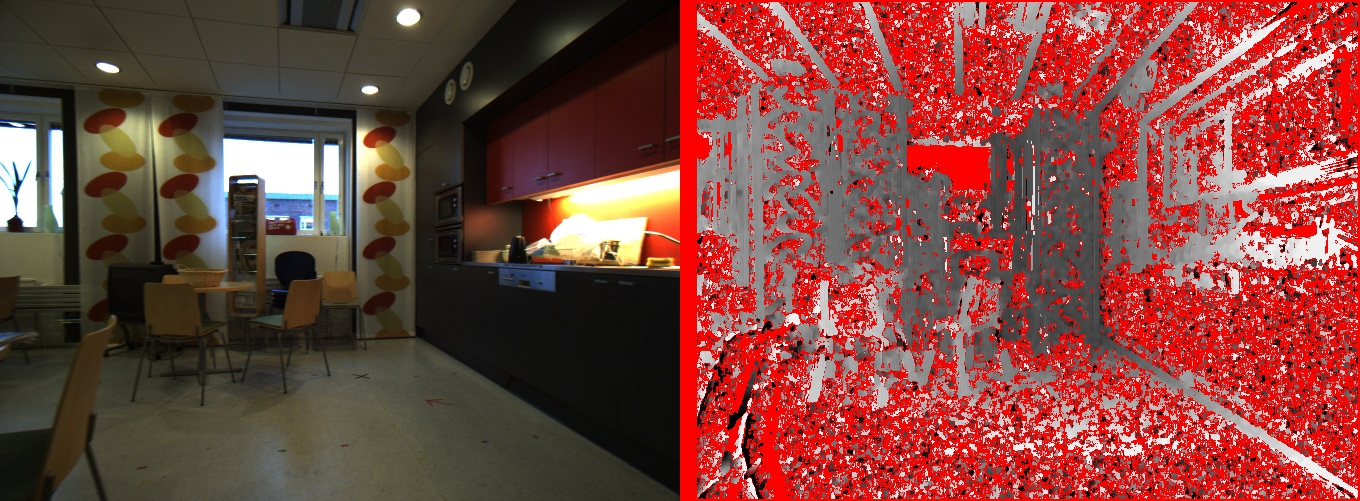
\includegraphics[width=\textwidth]{n_16_b_5}
	\caption{numDisparsities:16, blockSize:5}
\end{figure}

\begin{figure}[H]
	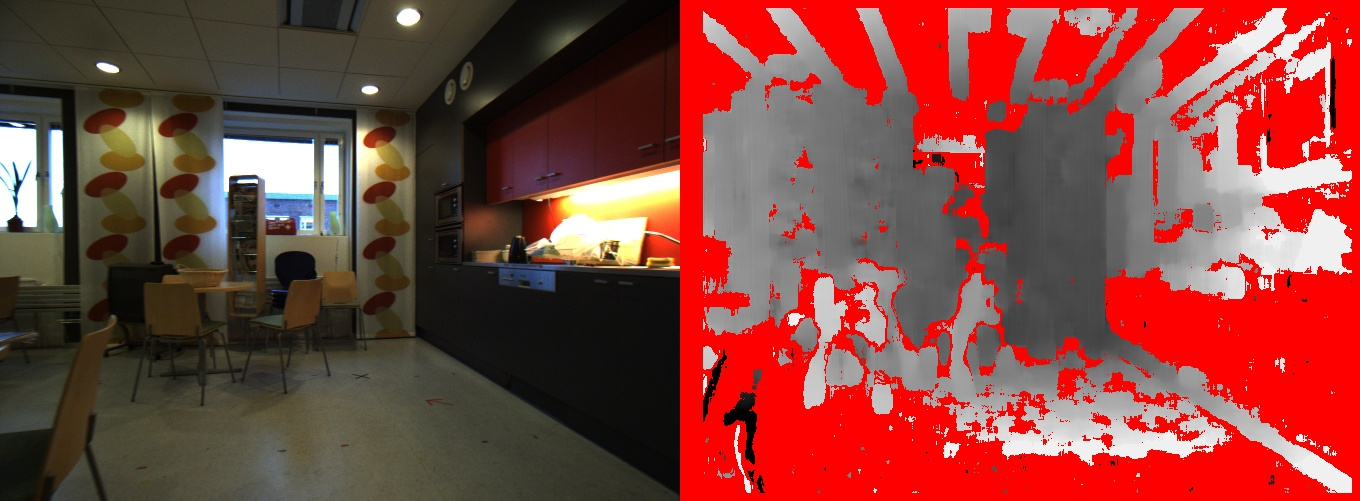
\includegraphics[width=\textwidth]{n_16_b_17}
	\caption{numDisparsities:16, blockSize:17}
\end{figure}

\begin{figure}[H]
	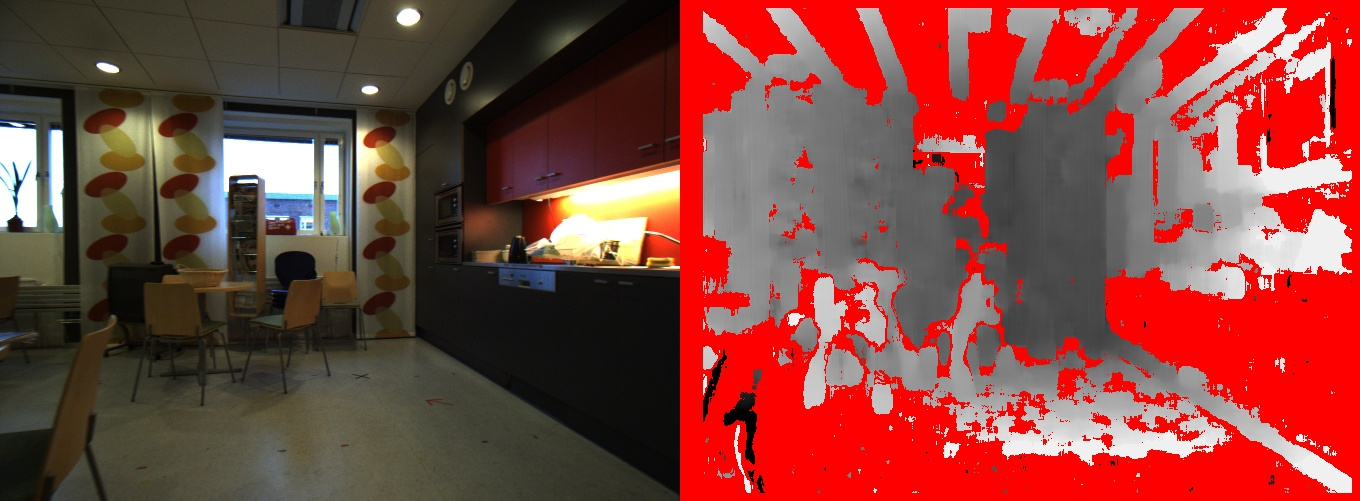
\includegraphics[width=\textwidth]{n_16_b_17}
	\caption{numDisparsities:16, blockSize:51}
\end{figure}

\begin{figure}[H]
	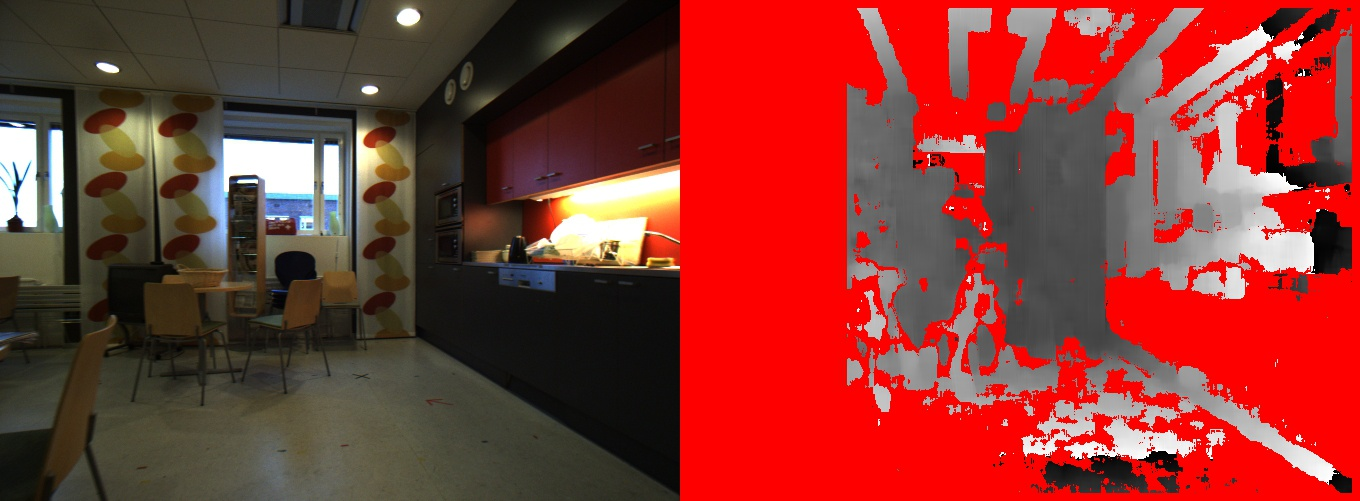
\includegraphics[width=\textwidth]{n_160_b_17}
	\caption{numDisparsities:160, blockSize:17}
\end{figure}

\clearpage

After that the algorithm SBGM was tested with different parameters. It detects more matching points. It also produce better objects' contours at result figure. For the figure, where cameras look at lift's wall SBGM allows to calculate disparity for more pixels. Table 1 shows the set of parameters, which was used (the set was found in the internet and then tuned for this set of frames). An area with negative results on the left side of image exists regardless of SBGM settings (at least those settings, which were tested).
\\
\\
\begin{tabular}{| p{3cm} | p{7cm} | p{3cm} |}
\hline
Parameter & Value & Comment \\
\hline
numDisparsities & 32 & \\
\hline
blockSize & 17 & \\
\hline
P1 & 200 & Increasing of this parameter increases amount of negative results\\
\hline
P2 & 500 & \\
\hline
disp12MaxDiff & 20 & Increasing this parameter's value reduce amount of negative results. But there was no much sense to set it larger, than 20, as gain was indistinguishable\\
\hline
preFilterCap & 20 & \\
\hline
uniquenessRatio & 1 & \\
\hline
speckleWindowSize & 0 & \\
\hline
speckleRange & 0 & \\
\hline
mode & STEREO\_SGBM\_MODE\_SGBM\_3WAY & SGBM 3Way version \\
\hline
\end{tabular}

\begin{figure}[H]
	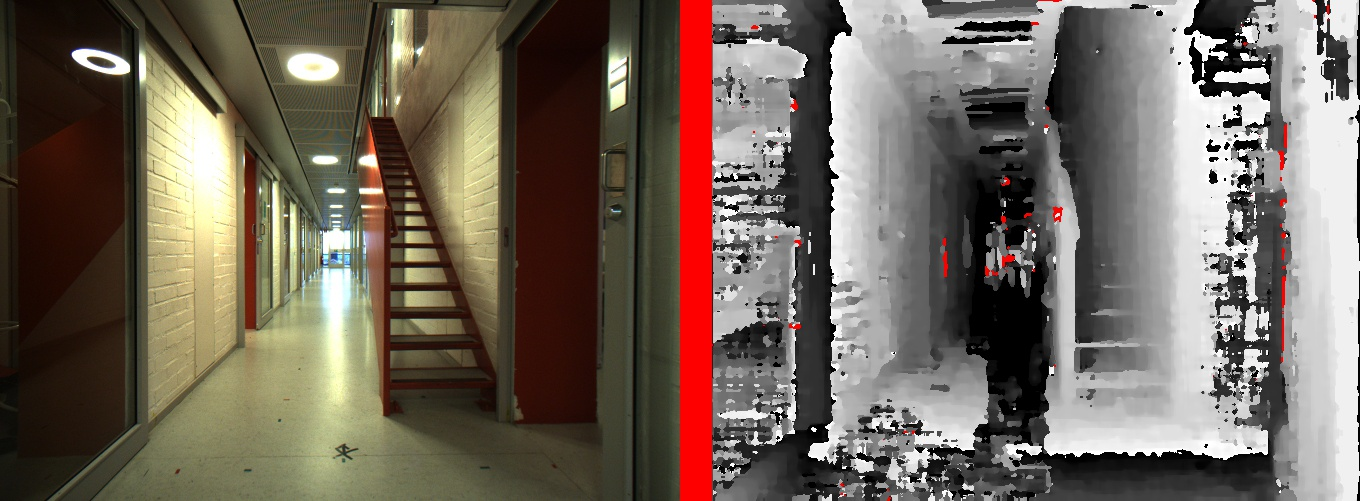
\includegraphics[width=\textwidth]{sbgm1}
	\caption{Corridor with stairs}
\end{figure}

\begin{figure}[H]
	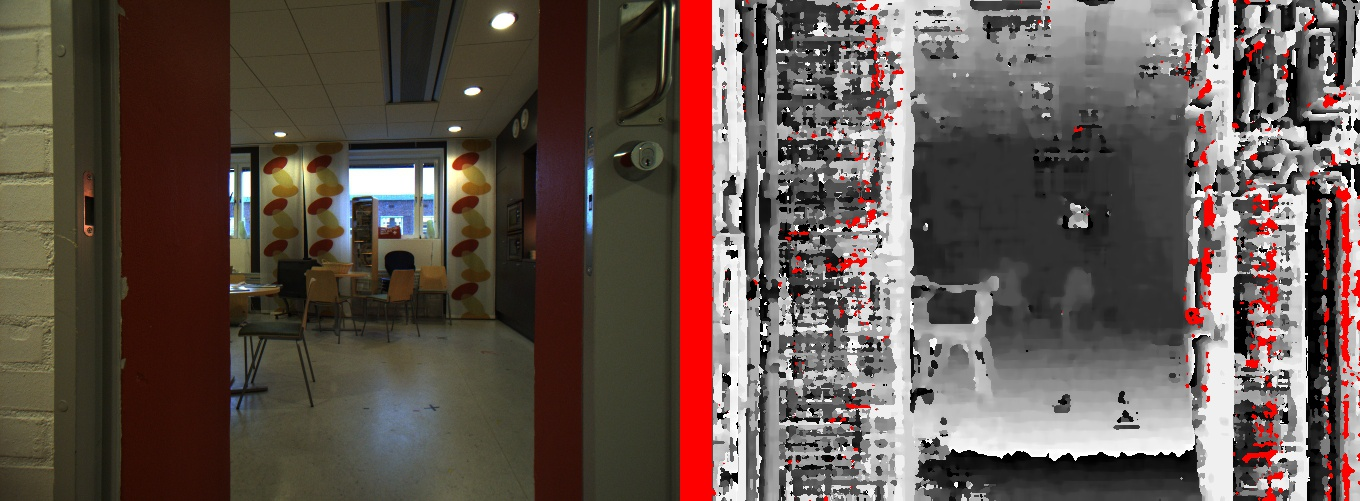
\includegraphics[width=\textwidth]{sbgm2}
	\caption{Entrance to a room}
\end{figure}

\begin{figure}[H]
	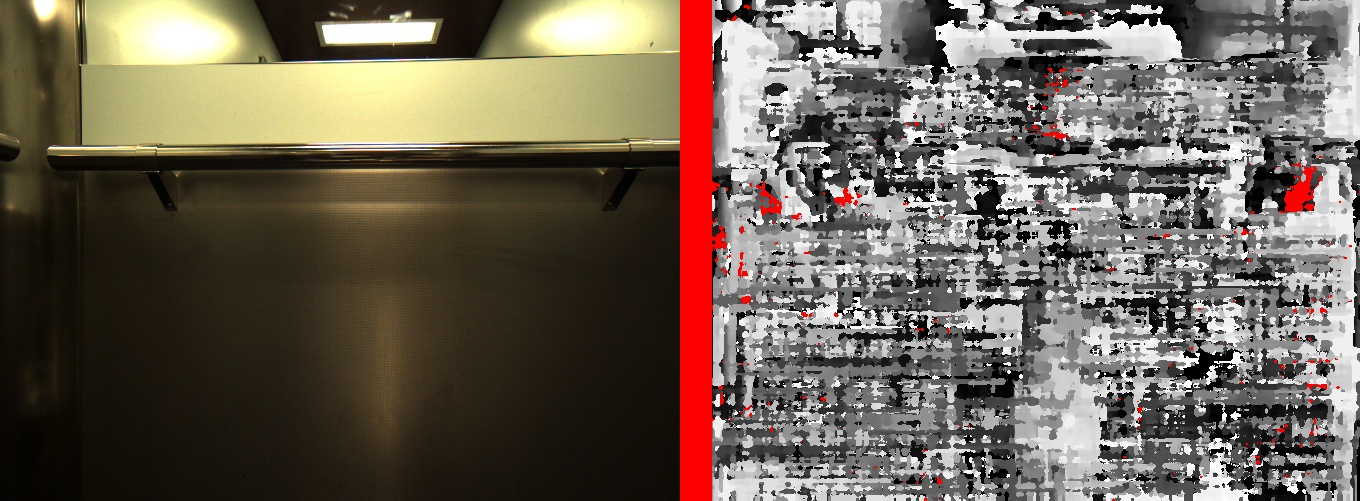
\includegraphics[width=\textwidth]{sbgm3}
	\caption{Lift's wall}
\end{figure}

\end{document}
%  LocalWords:  Jorma Laaksonen pdf py tex OpenCV libopencv dev jpg
%  LocalWords:  highgui imgproc imgcodecs greyscale png opencv ing
%  LocalWords:  texlive includegraphics Exactum Gür Ersalan
